%
% chapter.tex -- Zusammenhang und kovariante Ableitung
%
% (c) 2025 Prof Dr Andreas Müller
%
\chapter{Zusammenhang und kovariante Ableitung
\label{chapter:zusammenhang}}
\kopflinks{Zusammenhang und kovariante Ableitung}

\noindent
Die Diskussion der Lie-Ableitung in
Abschnitt~\ref{buch:koordinaten:section:differentialoperatoren}
hat gezeigt, dass die zweite Ableitung eines Kurve nicht auf
allgemein kovariante Art definiert werden kann.
Der Grund dafür ist, dass die Tangentialvektoren in den Punkten
$\gamma(t)$ und $\gamma(t+\Delta t)$ in den disjunkten Vektorräumen
$T_{\gamma(t)}M$ und $T_{\gamma(t+\Delta t)}M$ liegen und sich nicht
einfach so miteinander verrechnen lassen.
Dazu wird eine Methode benötigt, die Tangentialvektoren vom einen
Punkt in einen nahegelegenen Punkt zu transportieren.
Die einfachste Methode, dies zu erreichen, ist eine Metrik $g$ auf der
Mannigfaltigkeit zu verwenden, und Vektoren ``parallel'' zu transportieren,
wie dies in Abschnitt~\ref{buch:zusammenhang:section:paralleltransport}
unternommen wird.
{\em Geodäten} sind kürzeste Verbindungen auf einer Mannigfaltigkeit, sie
lassen sich aber auch als Kurven charakterisieren, die ihren Tangentialvektor
parallel transportieren.
\index{Geodäte}%
Dies definiert eine Differentialgleichung zweiter Ordnung für die
Geodäten (Abschnitt~\ref{buch:zusammenhang:section:geodaeten}).
Die kovariante Ableitung von
Abschnitt~\ref{buch:zusammenhang:section:kovarianteableitung}
verallgemeinert den Differentialoperator, der in der Differentialgleichung
der Geodäten vorkommt, für beliebige Vektoren.
Die kovariante Ableitung ist festgelegt, wenn man auf der Mannigfaltigkeit
eine sogenannten {\em Zusammenhang} definiert hat
(Abschnitt~\ref{buch:zusammenhang:section:zusammenhang}). 
\index{Zusammenhang}%
In Abschnitt~\ref{buch:zusammenhang:section:paralleltransport} wurden
Vektoren mit Hilfe des Paralleltransports verglichen.
Ein Zusammenhang verallgemeinert diese Idee und ermöglicht damit auch
Vektoren zu vergleichen, die nicht mit der Metrik verrechnet werden
können.

%
% Paralleltransport
%
\section{Paralleltransport
\label{buch:zusammenhang:section:paralleltransport}}
In diesem Abschnitt versuchen wir ein Kriterium zu finden, welches
entscheidet, ob ein Vektor entlang einer Kurve parallel transportiert
worden ist.
Da auch dies eine Eigenschaft sein muss, die sich lokal entscheiden
lässt, muss das Kriterium in form einer Differentialgleichung
formuliert werden können.
Der zugehörige Differentialausdruck ist die kovariante Ableitung,
die in Abschnitt~\ref{buch:zusammenhang:subsection:paralleltransport}
vorgestellt wird.
Die darin auftretenden Koeffizienten sind die {\em Christoffel-Symbole},
die in Abschnitt~\ref{buch:zusammenhang:subsection:paralleltransport}
berechnet werden.

%
% Kovariante Ableitung
%
\subsection{Kovariante Ableitung
\label{buch:zusammenhang:subsection:paralleltransport}}
Wir betrachten ein Vektorfeld $A(x)\in T_xM$ auf der Mannigfaltigkeit 
und versuchen ein Kriterium zu finden, wie sich die Komponenten
ändern, wenn der Vektor parallel transportiert wird.
Da die Betrachtungen lokal sind, können wir den Vektor in einem
lokalen Koordinatensystem durch seine Komponenten $A^i$ mit
\[
A(x) = \sum_{i=1}^n A^i(x)\vec{e}_i
\]
ausdrücken.
Im Folgenden werden wir das Argument $x$ der Einfachheit halber
jeweils weglassen.

Wir bestimmen jetzt die Einflüsse, nach denen sich die Komponenten
$A^i$ ändern, wenn man sich im Vektorfeld in Richtung eines
Vektors $X$ mit den Komponenten $\xi^k$ verschiebt.
Die partiellen Ableitungen hängen von den Koordinaten ab und haben
daher auch dann von $0$ verschiedene partielle Ableitungen nach
den Koordinaten, wenn der Vektor parallel verschoben wird.
Diese Ableitungen sind auch bei einem parallel transportierten
Vektor gross, wenn die Koordinatenlinien stark gekrümmt sind.
Die partiellen Ableitungen können daher nicht das alleinige Kriterium
für Paralleltransport sein.

Zu den Änderungen der Komponenten in Abhängigkeit von den Koordinaten
kommt ein weiterer Term hinzu, so dass wir die $i$-te Komponte der Änderung
des transportierten Vektors als
\begin{equation}
\sum_{k=1}^n
\frac{\partial A^i}{\partial x^k}
\xi^k
+
\Gamma^i(A,X)
\label{buch:zusammenhang:paralleltransport:eqn:kovabl}
\end{equation}
schreiben können.

Die Summe der paralletransportierten Vektoren soll in den
paralleltransportierten Summenvektor übergehen.
Das Kriterium für Paralleltransport muss daher linear in $A$ sein.
Die partiellen Ableitungen nach den Koordinaten sind bereits linear
in $A$, daher muss auch $\Gamma^i(A,X)$ linear in $A$ sein.
Da der Ausdruck
\eqref{buch:zusammenhang:paralleltransport:eqn:kovabl}
die Änderung für eine infinitesimale Verschiebung in Richtung
des Vektors $X$ angeben soll, muss $\Gamma^i(A,X)$ linear
von den Komponenten $\xi^k$ von $X$ abhängen.
Somit lässt er sich in der Form
\begin{equation}
\frac{\partial A^i}{\partial x^k}\xi^k
+
\Gamma^i_{lk}(x)A^l\xi^k
\end{equation}
schreiben, wobei die Koeffizienten $\Gamma^i_{lk}(x)$ natürlich
von den Koordinaten abhängen können.

\begin{definition}[kovariante Ableitung]
\label{buch:zusammenhang:paralleltransport:kovabl:def:kovabl}
Die {\em kovariante Ableitung} eines Vektorfeldes $A$ mit Koponenten $A^i$
\index{kovariante Ableitung}%
\index{Ableitung!kovariant}%
in Richtung eines Vektors $X$ mit den Komponenten $\xi^k$ ist
\begin{equation}
\nabla_X A
=
\sum_{k=1}^n
(\nabla_k A)
\xi^k
=
\sum_{i=1}^n
\biggl(
\sum_{k=1}^n
(
\nabla_k A^i
)
\xi^k
\biggr)
\,
\vec{e}_i
=
\sum_{i,k=1}^n
\biggl(
\frac{\partial A^i}{\partial x^k}
+
\Gamma^{i}_{lk} A^l
\biggr)
\,
\xi^k
\,
\vec{e}_i
\label{buch:zusammenhang:paralleltransport:eqn:koverianteableitung}
\end{equation}
Die Koeffizienten $\Gamma^i_{lk}$ heissen die {\em Christoffel-Symbole}.
\index{Christoffel-Symbole}%
\end{definition}

Für die Richtung $\vec{e}_k$ der $k$-ten Koordinaten $x^k$, kann man die
kovariante Ableitung
\[
\frac{\partial A^i}{\partial x^k}
+
\sum_{l=1}^n
\Gamma^i_{lk} A^l
\]
auch in Matrixform als
\[
\nabla_k A
=
\frac{\partial}{\partial x^k}
\begin{pmatrix}
A^1\\[-2pt]
\vdots\\
A^n
\end{pmatrix}
+
\begin{pmatrix}
\Gamma_{1k}^1 & \dots  & \Gamma^1_{nk} \\[-2pt]
\vdots        & \ddots & \vdots \\
\Gamma_{1k}^n & \dots  & \Gamma^n_{nk} \\
\end{pmatrix}
\begin{pmatrix}
A^1\\[-2pt]
\vdots\\
A^n
\end{pmatrix}
\]
schreiben.
Die kovariante Ableitung ist somit gegeben durch eine linear von $X$
abhängige Matrix 
\[
\sum_{k=1}^n \xi^k \Gamma_k
\quad
\text{mit}
\quad
\Gamma_k
=
\begin{pmatrix}
\Gamma_{1k}^1 & \dots  & \Gamma^1_{nk} \\[-2pt]
\vdots        & \ddots & \vdots \\
\Gamma_{1k}^n & \dots  & \Gamma^n_{nk} \\
\end{pmatrix}
\]
in der Form
\[
\nabla_X A
=
\sum_{k=1}^n
\xi^k
\biggl(
\frac{\partial}{\partial x^k}
+
\Gamma_k
\biggr)\, A.
\]
Die Matrix $\Gamma_k$ gibt also an, wie die durch Krümmung der
Koordinatenlinien bedingten Änderungen der Komponenten $A^i$ 
kompensiert werden müssen.

\begin{definition}[paralleltransportiertes Vektorfeld]
Ein Vektorfeld $A^i$ heisst paralleltransportiert entlang der Richtung
$X$ mit Komponenten $\xi^k$, wenn die kovariante Ableitung
\begin{equation*}
\nabla_X A
=
\sum_{i,k=1}^n
\xi^k
\biggl(
\frac{\partial A^i}{\partial x^k}
+
\sum_{l=1}^n
\Gamma^i_{lk} A^l
\biggr)
\,\vec{e}_i
= 0
\end{equation*}
verschwindet.
\end{definition}

In einem $n$-dimensionalen euklidischen Raum mit kartesischen Koordinaten
sind die paralleltransportierten Vektorfelder leicht zu identifizieren,
es sind die Vektorfelder mit konstanten Komponenten.
In diesem Falle verschwinden die partiellen Ableitungen.

%
% Kovariante Ableitung der Standardbasisvektoren in einer Karte
%
\subsubsection{Kovariante Ableitung der Standardbasisvektoren in einer Karte}
Für die Standardbasisvektoren $\vec{e}_j$ in einer Karte sind die
Komponenten $\delta_j^k$.
Die kovarianten Ableitungen von $\vec{e}_j$ ist daher
\begin{equation}
\nabla_X\cdot \vec{e}_j
=
\xi^k
\biggl(
\frac{\partial \delta_j^i}{\partial x^k}
+
\Gamma^i_{lk}
\delta_j^l
\biggr)
\vec{e}_i
=
\xi^k\Gamma^i_{jk}\vec{e}_i
\label{buch:zusammenhang:paralleltransport:kovabl:eqn:kontravektor}
\end{equation}
oder
\begin{equation}
\nabla_{\vec{e}_k}\cdot \vec{e}_j
=
\sum_{i=1}^n
\Gamma^i_{jk}\vec{e}_i
\label{buch:zusammenhang:paralleltransport:kovabl:eqn:kontrabasis}
\end{equation}
Die Christoffel-Symbole in einer Karte beschreiben daher die Komponenten
der kovarianten Ableitung der Standardbasisvektoren in Richtung
der Standardbasisvektoren.
%
% Koordinatentransformation für Christoffel-Symbole
%
\subsubsection{Koordinatentransformation für Christoffel-Symbole}
Die Christoffel-Symbole bilden keinen Tensor dritter Stufe.
Wären Sie ein Tensor, dann würde $A\mapsto \Gamma(A,X)$ eine lineare
Abbildung von Vektoren definieren, $\Gamma(A,X)$ wäre ein Vektor.
Da die kovariante Ableitung $\nabla_XA$ ein Vektor sein soll,
die zweiten Ableitungen der Komponenten eines Vektors aber kein Vektor
sein können, können auch die Christoffel-Symbole keinen Tensor bilden.
In diesem Abschnitt soll daher das Transformationsgesetz für die
Christoffel-Symbole bei einem Koordinatenwechsel bestimmt werden.

Seien also $A^i$ und $\xi^k$ die Komponenten eines (kontravarianter)
Vektoren im $x^i$-Koor\-di\-na\-ten\-system.
Sie sollen jetzt umgerechnet werden in ein $y^i$-Koordinatensystem, in
das Vektorkomponenten mit der Jacobi-Matrix
\[
J^i\mathstrut_k
=
\frac{\partial (y^1,\dots,y^n)}{\partial(x^1,\dots,x^n)}
\]
umgerechnet werden können.
Die Komponenten des Vektors $A$ im $y$-Koordinatensystem bezeichnen
wir mit $\tilde{A}^i$, jene von $X$ mit $\tilde{\xi}^i$.
Die transformierten Christoffel-Symbole $\tilde{\Gamma}^i_{lk}$ müssen
die transformierten komponenten der kovarianten Ableitung liefern.

Einsetzen der transformierten Komponenten in die kovariante Ableitung
im $y$-Koor\-di\-na\-ten\-system ergibt unter Verwendung der einsteinschen
Summationskonvention
\begin{align}
\tilde{\xi}^k
\biggl(
\frac{\partial}{\partial y^k}
\tilde{A}^i
+
\tilde{\Gamma}^i_{lk}\tilde{A}^l
\biggr)
&=
J^k\mathstrut_u
\xi^u
\biggl(
\frac{\partial}{\partial y^k}
(J^i\mathstrut_r A^r)
+
\tilde{\Gamma}^i_{lk} J^l\mathstrut_rA^r
\biggr)
\notag
\\
&=
\xi^u\biggl(
J^k_u\frac{\partial}{\partial y^k}
(J^i\mathstrut_r A^r)
+
\tilde{\Gamma}^i_{lk}
J^k\mathstrut_u 
J^l\mathstrut_r
A^r
\biggr)
\notag
\\
&=
\xi^u\biggl(
\frac{\partial}{\partial x^u}
(J^i\mathstrut_r A^r)
+
\tilde{\Gamma}^i_{lk}
J^k\mathstrut_u 
J^l\mathstrut_r
A^r
\biggr)
\notag
\\
&=
\xi^u
\biggl(
\frac{\partial J^i\mathstrut_r}{\partial x^u}A^r
+
J^i\mathstrut_s\frac{\partial A^s}{\partial x^u}
+
\tilde{\Gamma}^i_{lk}
J^l\mathstrut_r
J^k\mathstrut_u
A^r
\biggr)
\notag
\\
&=
\xi^u
\biggl(
J^i\mathstrut_s\frac{\partial A^s}{\partial x^u}
+
\frac{\partial J^i\mathstrut_r}{\partial x^u}A^r
+
\tilde{\Gamma}^i_{lk}
J^l\mathstrut_r
J^k\mathstrut_u
A^r
\biggr)
\notag
\\
&=
\xi^u
J^i\mathstrut_s\frac{\partial A^s}{\partial x^u}
+
\xi^u
\biggl(
\frac{\partial J^i\mathstrut_r}{\partial x^u}
+
\tilde{\Gamma}^i_{lk}
J^l\mathstrut_r
J^k\mathstrut_u
\biggr)
\,A^r.
\label{buch:zusammenhang:paralleltransport:eqn:gammatilde}
\intertext{Transformiert man dagegen die Komponenten der kovariante Ableitung
im $x$-Koordinaten\-system mit $J^i\mathstrut_k$, erhält man}
&=
\xi^u
J^i\mathstrut_s\biggl(
\frac{\partial A^s}{\partial x^u}
+
\Gamma^s_{ru} A^r
\biggr)
\notag
\\
&=
\xi^u
J^i\mathstrut_s
\frac{\partial A^s}{\partial x^u}
+
\xi^u
J^i\mathstrut_s
\Gamma^s_{ru} A^r.
\label{buch:zusammenhang:paralleltransport:eqn:gamma}
\end{align}
Der Vergleich von
\eqref{buch:zusammenhang:paralleltransport:eqn:gammatilde}
mit
\eqref{buch:zusammenhang:paralleltransport:eqn:gamma}
ergibt das Transformationsgesetz
\begin{align*}
\frac{\partial J^i\mathstrut_r}{\partial x^u}
+
\tilde{\Gamma}^i_{lk}
J^l\mathstrut_r
J^k\mathstrut_u
=
J^i\mathstrut_s
\Gamma^s_{ru},
\end{align*}
welche wie erwartet zweite Ableitungen der Einträge der Jacobi-Matrix
enthält.
Multipliziert man mit der Inversen $J_i\mathstrut^t$ der Jacobi-Matrix,
erhält man
\begin{align*}
J_i\mathstrut^t
\frac{\partial J^i\mathstrut_r}{\partial x^u}
+
J_i\mathstrut^t
\tilde{\Gamma}^i_{lk}
J^l\mathstrut_r
J^k\mathstrut_u
=
J_i\mathstrut^t
J^i\mathstrut_s
\Gamma^s_{ru}
=
\delta^t_s
\Gamma^s_{ru}
=
\Gamma^t_{ru}.
\end{align*}
Die Transformation der Christoffel-Symbole erfolgt daher wie erwartet
für jeden oberen und unteren Index, aber es kommt noch ein Term mit
den zweiten Ableitungen der Jacobi-Matrix hinzu.

%
% Kovariante Ableitung für $p$-Vektoren
%
\subsubsection{Kovariante Ableitung für kontravariante Tensoren}
Die kovariante Ableitung ist in
Definition~\ref{buch:zusammenhang:paralleltransport:kovabl:def:kovabl}
nur für einzelne Vektoren, also kontravariante Tensoren erster Stufe,
definiert.
Es gibt nur eine Art, sie auf kontravariante Tensoren beliebiger Stufe
auszudehnen, so dass die Produktregel gilt.

\begin{definition}
Die kovariante Ableitung eines $p$-Vektors $X_1\otimes\dots\otimes X_p$
ist
\[
\nabla_X\cdot (X_1\otimes\dots\otimes X_p)
=
\sum_{i=1}^p
X_1\otimes\dots\otimes(\nabla_X\cdot X_i)\otimes\dots X_p.
\]
\end{definition}

Für einen beliebigen Tensor $p$-ter Stufe der Form
\[
a
=
a^{i_1\dots i_p}
X_{i_1}\otimes\dots\otimes X_{i_p}
\]
muss die kontravariante Ableitung nach der Produktregel
\begin{align*}
\nabla_X\cdot a
&=
\sum_{i_1,\dots,i_p=1}^n
\biggl(
(X\cdot a^{i_1\dots i_p}) X_{i_1}\otimes\dots\otimes X_{i_p}
+
a_{i_1\dots i_p}
\sum_{k=1}^n
X_{i_1}\otimes\dots\otimes(\nabla_X X_{i_k})\otimes\dots\otimes X_{i_p}
\biggr)
\end{align*}
sein.
Schreibt man den Tensor $a$ in der Basis der Tensorprodukt von
Standarbasisvektoren $e_{i_1}\otimes\dots\otimes e_{i_p}$ als
\[
a
=
\sum_{i_1,\dots,i_p}
a^{i_1\dots i_p}
(e_{i_1}\otimes\dots\otimes e_{i_p}),
\]
dann ist die kovariante Ableitung
\begin{align*}
\nabla_{\vec{e}_k} \cdot a
&=
\sum_{i_1,\dots,i_p=1}^n
\biggl(
\frac{\partial a^{i_1\dots i_p}}{\partial x^k}
(\vec{e}_{i_1}\otimes\dots\otimes\vec{e}_{i_p})
+
a^{i_1\dots i_p}
\sum_{j=1}^p
\vec{e}_{i_1}\otimes\dots\otimes(\nabla_{\vec{e}_k}\cdot\vec{e}_{i_j})\otimes\dots\otimes \vec{e}_{i_p}
\biggr)
\\
&=
\sum_{i_1,\dots,i_p=1}^n
\biggl(
\frac{\partial a^{i_1\dots i_p}}{\partial x^k}
(\vec{e}_{i_1}\otimes\dots\otimes\vec{e}_{i_p})
+
a^{i_1\dots i_p}
\sum_{j=1}^p
\Gamma^i_{i_jk}
\sum_{i=1}^n
(\vec{e}_{i_1}\otimes\dots\otimes \vec{e}_i \otimes\dots\otimes \vec{e}_{i_p})
\biggr).
\end{align*}
Die Koeffizienten von $\nabla_{\vec{e}_k}\cdot a$ sind
\begin{equation}
\frac{\partial a^{i_1\dots i_p}}{\partial x^k}
+
a^{li_2\dots i_p}
\Gamma^{i_1}_{lk}
+
\dots
+
a^{i_1\dots i_{p-1}l}
\Gamma^{i_p}_{lk}
=
\frac{\partial a^{i_1\dots i_p}}{\partial x^k}
+
\sum_{j=1}^p
a^{i_1\dots l\dots i_p}
\Gamma^{i_j}_{lk}.
\label{buch:zusammenhang:kovabl:eqn:ptensor}
\end{equation}
Zusätzlich zu den partiellen Ableitungen wird jeder Index von
$a^{i_1\dots i_p}$ mit einem Ausdruck mit Christoffel-Symbolen
Transformiert.
Für $p=1$ entsteht aus 
\eqref{buch:zusammenhang:kovabl:eqn:ptensor}
die bekannte Formel für die kovariante Ableitung eines Vektors.

%
% Kovariante Ableitung beliebiger Tensoren
%
\subsubsection{Kovariante Ableitung beliebiger Tensoren}
Die Formel~\eqref{buch:zusammenhang:paralleltransport:eqn:koverianteableitung}
für die kovariante Ableitung funktioniert nur für Vektoren.
Für Ableitung einer Funktion $f$ entlang einer Richtung ändert
die Metrik nichts, diese Ableitung $X\cdot f$ ist daher die bereits
bekannte Ableitung $X\cdot f = \langle df,X\rangle$.
Die kovariante Ableitung einer Funktion unterscheidet sich daher nicht
von Richtungsableitung.

Für eine 1-Form $\alpha$ lässt sich jetzt auch eine kovariante Ableitung
$\nabla_X\alpha$ so definieren, dass die Produktregel gilt, dass also
\[
\nabla_X
\langle \alpha, A\rangle
=
\langle \nabla_X\alpha,A\rangle
+
\langle \alpha,\nabla_X A\rangle
\]
gilt.
Durch Aufläsen nach dem ersten Term auf der rechten Seite erhält man
\begin{equation}
\langle \nabla_X\alpha,A\rangle
=
X
\cdot
\langle \alpha, A\rangle
-
\langle \alpha,\nabla_X A\rangle.
\label{buch:zusammenhang:paralleltransport:eqn:kovariant}
\end{equation}
In einer Karte wird 
\eqref{buch:zusammenhang:paralleltransport:eqn:kovariant}
zu
\begin{align*}
\langle
\nabla_X\cdot\alpha, A
\rangle
&=
\xi^k
\frac{\partial}{\partial x^k} (a_i A^i)
-
a_i
\biggl(
\frac{\partial A^i}{\partial x^k}
+
\Gamma^i_{rk} A^r
\biggr)
\xi^k
\\
&=
\biggl(
A^i
\frac{\partial a_i}{\partial x^k}
+
a_i
\frac{\partial A^i}{\partial x^k}
-
a_i
\frac{\partial A^i}{\partial x^k}
-
a_i
\Gamma^i_{rk} A^r
\biggr)
\xi^k
\\
&=
\xi^k A^r
\biggl(
\frac{\partial a_r}{\partial x^k}
-
\Gamma^i_{rk}a_i
\biggr).
\end{align*}
Da dies für alle Vektoren $A$ und $X$ gelten muss, 

\begin{definition}[kovariante Ableitung von 1-Formen]
Ist $\nabla_X$ die kovariante Ableitung von kontravarianten
Tensoren erster Stufe in Richtung des Vektors $X$ mit den
Christoffel-Symbolen $\Gamma^i_{kl}$,
dann ist die kovariante Ableitung
der 1-Form $\alpha$ eine 1-Form
\[
\nabla_k\cdot\alpha
=
\sum_{r=1}^n
\biggl(
\frac{\partial a_r}{\partial x^k} - \Gamma^i_{rk}a_i
\biggr)
\,dx^r
\]
mit den Komponenten
\[
(\nabla_k\cdot\alpha)_r
=
\frac{\partial a_r}{\partial x^k} - \Gamma^i_{rk}a_i
\]
\end{definition}

Ganz ähnlich wie bei der kovarianten Ableitung von kontravarianten
Tensoren $p$-ter Stufe lässt sich jetzt auch die kovariante
Ableitung eines kovarianten Tensors definieren.
Für die Komponenten der kovarianten Ableitung werden zur partiellen
Ableitung der Komponenten für jeden kontravarianten Index $i_j$ der
Komponenten $a_{\dots i\dots}$ mit $-\Gamma^{i}_{i_jk}$ multipliziert
und über $i$ summiert.

%
% Christoffel-Symbole
%
\subsection{Berechnung der Christoffel-Symbole
\label{buch:zusammenhang:subsection:christoffel}}
Wir haben die Entwicklung der kovarianten Ableitung mit der Idee des
Paralleltransportes motiviert.
Dabei haben wir implizit an die Vorstellung appelliert, dass es
möglich ist, Länge und Richtung eines Tangentialvektors zu beurteilen.
Dies geht aber nur, wenn auf der Mannigfaltigkeit auch eine Metrik
gegeben ist.
Erst durch die Vorgabe einer Metrik wird es daher auch möglich, die
Christoffel-Symbole explizit zu bestimmen, was in diesem Abschnitt
geschehen soll.

%
% Kovariante Ableitung des metrischen Tensors
%
\subsubsection{Kovariante Ableitung des metrischen Tensors}
Sei also eine Metrik als symmetrischer, kovarianter Tensor zweiter Stufe
mit den Koeffikzenten $g_{ik}(x)$.
Durch die Koeffizienten $g_{ik}$ wird das Skalarprodukt
\[
g(A,B)
=
\langle A,B\rangle_g
=
\langle A,B\rangle
=
g_{ik} A^i B^k
\]
(einsteinsche Summationskonvention)
von Tangentialvektoren $A$ und $B$ definiert.
Die kovariante Ableitung soll so konstruiert werden, dass die
kovariante Ableitung des Tensors $g$ verschwindet, also $\nabla_X\cdot g=0$.
Aus der Produktregel folgt dann, dass
\[
\nabla_X\cdot g(A,B)
=
g(\nabla_X\cdot A, B)
+
g(A,\nabla_X\cdot B)
\]
gilt.
Für den Vektor $X=\vec{e}_k$ bekommt dies die Form
\begin{align}
\nabla_{\vec{e}_k}\cdot g(A,B)
&=
\frac{\partial}{\partial x^k} g_{il}A^iB^l
\notag
\\
&=
\frac{\partial g_{il}}{\partial x^k} A^iB^l
+
g_{il}\frac{\partial A^i}{\partial x^k} B^l
+
g_{il}A^i\frac{\partial B^l}{\partial x^k}
\notag
\\
g(\nabla_{\vec{e}_k}\cdot A, B)
&=
g_{il}\biggl(\frac{\partial A^i}{\partial x^k} + \Gamma^i_{sk}A^s \biggr) B^l
\notag
\\
g(A,\nabla_{\vec{e}_k}\cdot B)
&=
g_{il}A^i\biggl(
\frac{\partial B^l}{\partial x^k}
+
\Gamma^l_{sk}B^s
\biggr)
\notag
\\
0&=
\frac{\partial g_{il}}{\partial x^k} A^iB^l
-g_{il}\Gamma^i_{sk}A^sB^l
-g_{il}\Gamma^l_{sk}A^iB^s
\notag
\intertext{Durch Umnummerieren der Summen über $i$ und $s$ mit mittleren
Term und $i$ und $s$ im rechten Term kann man erreichen, dass alle Terme
für $A$ und $B$ die gleichen Indizes verwenden.
Mit dem Ableitungsterm auf der linken Seite erhält man jetzt}
\frac{\partial g_{il}}{\partial x^k} A^iB^l
&=
\bigl(g_{sl}\Gamma^s_{ik} + g_{is}\Gamma^s_{lk}\bigr)A^iB^l.
\notag
\intertext{Da dies für alle Komponenten $A^i$ und $B^l$ gelten muss, kann
man diese weglassen und erhält.}
\frac{\partial g_{il}}{\partial x^k}
&=
g_{sl}\Gamma^s_{ik} + g_{is}\Gamma^s_{lk}.
\label{buch:zusammenhang:kovabl:eqn:gGamma}
\end{align}
Die Gleichung
\eqref{buch:zusammenhang:kovabl:eqn:gGamma}
stellt einen Zusammenhang zwischen den Christoffel-Symbolen und
dem metrischen Tensor her.

%
% Lösung des Gleichungssystems
%
\subsubsection{Lösung des Gleichungssystems
\eqref{buch:zusammenhang:kovabl:eqn:gGamma}}
Durch zyklische Vertauschung der Indizes $i$, $k$ und $l$ ergeben sich
die Gleichungen
\begin{equation}
\renewcommand{\arraystretch}{2.0}
\renewcommand{\arraycolsep}{2pt}
\left.
\begin{array}{rcrcrcl}
\displaystyle\frac{\partial g_{il}}{\partial x^k}
&=&
g_{sl}\Gamma^s_{ik}
&+&
g_{is} \Gamma^s_{lk}
& &
\\
\displaystyle\frac{\partial g_{ki}}{\partial x^l}
&=&
& &
g_{si} \Gamma^s_{kl}
&+&
g_{ks}\Gamma^s_{il}
\\
\displaystyle\frac{\partial g_{lk}}{\partial x^i}
&=&
g_{ls} \Gamma^s_{ki}
& &
&+&
g_{sk}\Gamma^s_{li}.
\end{array}
\quad
\right\}
\label{buch:zusammenhang:kovabl:eqn:gGammgl}
\end{equation}
Da $g$ symmetrisch ist, spielt die Reihenfolge der Indizes von $g$ keine
Rolle.
In den Christoffel-Symbolen treten ebenfalls verschiedene Reihenfolgen
der beiden unteren Indizes auf.
Die Gleichungen bestimmen die Christoffel-Symbole nur, wenn zusätzliche
Annahmen über das Verhalten bei Vertauschung der unteren beiden
Indizes gemacht werden.
Wir nehmen daher an, dass $\Gamma$ in den unteren Indizes symmetrisch ist.
Dann vereinfachen sich die
Gleichungen~\eqref{buch:zusammenhang:kovabl:eqn:gGammgl}
zu
\begin{equation}
\renewcommand{\arraystretch}{2.0}
\renewcommand{\arraycolsep}{2pt}
\left.
\begin{array}{rcrcrcl}
\displaystyle\frac{\partial g_{il}}{\partial x^k}
&=&
g_{ls}\Gamma^s_{ik}
&+&
g_{is} \Gamma^s_{kl}
& &
\\
\displaystyle\frac{\partial g_{ki}}{\partial x^l}
&=&
& &
g_{is} \Gamma^s_{kl}
&+&
g_{ks}\Gamma^s_{il}
\\
\displaystyle\frac{\partial g_{lk}}{\partial x^i}
&=&
g_{ls} \Gamma^s_{ik}
& &
&+&
g_{ks}\Gamma^s_{il}.
\end{array}
\quad
\right\}
\label{buch:zusammenhang:kovabl:eqn:gGammgl}
\end{equation}
Subtrahiert man die mittlere Gleichung von der Summe der ersten und
der letzten, bleibt auf der rechten Seite nur der erste Term stehen,
nämlich
\begin{align}
\frac{\partial g_{il}}{\partial x^k}
+
\frac{\partial g_{lk}}{\partial x^i}
-
\frac{\partial g_{ki}}{\partial x^l}
&=
2g_{ls}\Gamma^s_{ik}
\notag
\intertext{Durch Multiplikation mit der inversen Matrix $g^{jl}$ und
summieren über $l$ ergibt sich wegen $g^{jl}g_{ls}=\delta^j_s$}
\Gamma^j_{ik}
&=
\frac12
g^{jl}
\biggl(
\frac{\partial g_{il}}{\partial x^k}
+
\frac{\partial g_{lk}}{\partial x^i}
-
\frac{\partial g_{ki}}{\partial x^l}
\biggr)
\label{buch:zusammenhang:kovabl:eqn:Gamma}
\end{align}
Diese Christoffel-Symbole sind auch bekannt als die Zusammenhangskoeffizienten
des Lévi-Cività-Zusammenhangs.
Die rechte Seite von \eqref{buch:zusammenhang:kovabl:eqn:Gamma} ohne die
inverse Matrix von $g$ ist auch bekannt als das {\em Christoffel-Symbol
erster Art}
\begin{equation}
\Gamma_{l,ik}
=
\frac12
\biggl(
\frac{\partial g_{il}}{\partial x^k}
+
\frac{\partial g_{lk}}{\partial x^i}
-
\frac{\partial g_{ki}}{\partial x^l}
\biggr)
.
\end{equation}
Zur klareren Unterscheidung werden die $\Gamma^i_{kl}$ oft auch die
Christoffel-Symbole zweiter Art genannt.

\begin{satz}
Der einzige Zusammenhang mit symmetrischen Christoffelsymbolen
$\Gamma^j_{ik}=\Gamma^j_{ki}$ ist der Lévi-Cività-Zusammenhang mit den
Zusammenhangskoeffizienten
\eqref{buch:zusammenhang:kovabl:eqn:Gamma}.
\end{satz}

%
% Beispiele
%
\subsubsection{Beispiele}

\begin{beispiel}
Für die Ebene mit kartesischen Koordinaten und der Standardmetrik
mit $g_{ik}=\delta_{ik}$ verschwinden alle Ableitungen der metrischen
Koeffizienten und damit verschwinden auch alle Christoffel-Symbole.
Die kovariante Ableitung $\nabla_X$ fällt in diesem Fall zusammen
mit der Richtungsableitung.
\end{beispiel}

\begin{beispiel}
\label{buch:zusammenhang:paralleltransport:bsp:polar}
In Polarkoordinaten $x^1=r$ und $x^2=\varphi$ in der Ebene ist die
Matrik durch die Matrix
\[
(g_{ik})
=
\begin{pmatrix}
1&0\\
0&r^2
\end{pmatrix}
\quad
\text{mit der Inversen}
\quad
(g^{jl})
=
\begin{pmatrix}
1&0\\
0&r^{-2}
\end{pmatrix}
\]
gegeben.
Nur die partiellen Ableitungen nach $x^1$ können überhaupt von $0$
verschieden sein.
Die einzige nicht verschwindende Ableitung ist
\[
\frac{\partial g_{22}}{\partial x^1}
=
2r.
\]
Daraus kann man bereits schliessen, dass die Christoffel-Symbole die Werte
$\pm\frac1r$ oder $\pm\frac2r$ haben müssen.
Die Christoffel-Symbole erster Art sind
\[
\begin{aligned}
\Gamma_{1,11} &= 0,
&
\Gamma_{1,12} &= \Gamma_{1,21} = 0,
&
\Gamma_{1,22} &= -r
\\
\Gamma_{2,11} &= 0,
&
\Gamma_{2,12} &= \Gamma_{2,21} = r,
&
\Gamma_{2,22} &= 0.
\end{aligned}
\]
Die Christoffel-Symbole zweiter Art sind dann durch
\[
\Gamma^j_{ik}
=
g^{jl}\Gamma_{l,ik}
=
g^{j1}\Gamma_{1,ik}
+
g^{j2}\Gamma_{2,ik}
=
\delta^{j1}\Gamma_{1,ik}
+
\frac{1}{r^2}
\delta^{j2}\Gamma_{2,ik}
=
\begin{cases}
\phantom{\frac1{r^2}}\Gamma_{1,ik}&\qquad\text{falls $j=1$}\\
         \frac1{r^2} \Gamma_{2,ik}&\qquad\text{falls $j=2$}
\end{cases}
\]
zu berechnen.
Es ergibt sich
\[
\begin{aligned}
\Gamma^1_{11} &= 0,
&
\Gamma^1_{21} &= \Gamma^1_{12} = 0,
&
\Gamma^1_{22} &= -r,
\\
\Gamma^2_{11} &= 0,
&
\Gamma^2_{21} &= \Gamma^2_{21} = \frac1r,
&
\Gamma^2_{22} &= 0.
\end{aligned}
\]
\end{beispiel}

\begin{beispiel}
\label{buch:zusammenhang:paralleltransport:bsp:kugel}
Kugelkoordinaten beschreiben Punkte der Einheitskugel mit Hilfe der
geographischen Länge und Breite 
\[
f\colon
[0,\pi] \times [0,2\pi)
\to
\mathbb{R}^3
:
(\vartheta,\varphi)
\mapsto
\begin{pmatrix}
\sin\vartheta \cos\varphi\\
\sin\vartheta \sin\varphi\\
\cos\vartheta
\end{pmatrix}
\]
Die geographische Breite wird vom Nordpol gemessen.
Die Komponenten des metrischen Tensors entstehen aus den Skalarprodukten
der partiellen Ableitungen nach $\vartheta$ und $\varphi$
\begin{align*}
\frac{\partial f}{\partial \vartheta}
&=
\begin{pmatrix}
\cos\vartheta \cos\varphi \\
\cos\vartheta \sin\varphi \\
-\sin\vartheta
\end{pmatrix}
&
\frac{\partial f}{\partial \varphi}
&=
\begin{pmatrix}
-\sin\vartheta\sin\varphi\\
 \sin\vartheta\cos\varphi\\
0
\end{pmatrix}.
\end{align*}
Sie sind
\begin{align*}
g_{11}
&=
\frac{\partial f}{\partial\vartheta}
\cdot
\frac{\partial f}{\partial\vartheta}
=
\cos^2\vartheta\cos^2\varphi+\cos^2\vartheta\sin^2\varphi+\sin^2\vartheta
\\
&=
\cos^2\vartheta(\underbrace{\cos^2\varphi+\sin^2\varphi}_{\displaystyle=1})+\sin^2\vartheta
=\cos^2\vartheta+\sin^2\vartheta=1
\\
g_{12}=g_{21}
&=
\frac{\partial f}{\partial\vartheta}
\cdot
\frac{\partial f}{\partial\varphi}
=
-\cos\vartheta\cos\varphi\sin\vartheta\sin\varphi
+\cos\vartheta\sin\varphi\sin\vartheta\cos\varphi
=
0
\\
g_{22}
&=
\frac{\partial f}{\partial\varphi}
\cdot
\frac{\partial f}{\partial\varphi}
=
\sin^2\vartheta\sin^2\varphi+\sin^2\vartheta\cos^2\varphi
=
\sin^2\vartheta(\underbrace{\sin^2\varphi+\cos^2\varphi}_{\displaystyle=1})
=
\sin^2\vartheta.
\end{align*}
Der metrische Tensor kann daher als die Matrix
\[
(g)
=
\begin{pmatrix}
1&0\\
0&\sin^2\vartheta
\end{pmatrix}
\]
geschrieben werden.

Ausgehend vom metrischen Tensor können jetzt auch die Christoffel-Symbole
berechnet werden.
Ganz ähnlich wie bei den Polarkoordinaten, sind
die partiellen Ableitungen nach $\vartheta$ von $g_{22}$ von $0$
verschieden:
\[
\frac{\partial g_{22}}{\partial x^1}
=
\frac{\partial g_{22}}{\partial\vartheta}
=
2\sin\vartheta\cos\vartheta.
\]
Die Christoffel-Symbole erster Art sind daher
\[
\begin{aligned}
\Gamma_{1,11}
&=
0,
&
\Gamma_{1,12} = \Gamma_{1,21}
&=
0,
&
\Gamma_{1,22}
&=
-\sin\vartheta\cos\vartheta,
\\
\Gamma_{2,11}
&=
0,
&
\Gamma_{2,12} = \Gamma_{2,21}
&=
\sin\vartheta\cos\vartheta,
&
\Gamma_{2,22}
&=
0.
\end{aligned}
\]
Mit der inversen Matrix von $g$ mit
\[
g^{ik}
=
\begin{pmatrix}
1&0\\
0&\frac{1}{\sin^2\vartheta}
\end{pmatrix}
\]
kann man jetzt auch die Christoffel-Symbole zweiter Art berechnen,
sie sind
\[
\Gamma^j_{ik}
=
g^{jl}\Gamma_{l,ik}
=
\begin{cases}
\Gamma_{1,ik}&\qquad\text{falls $j=1$}\\
\frac{1}{\sin^2\vartheta}\Gamma_{2,ik}&\qquad\text{falls $j=2$}.
\end{cases}
\]
Ausgerechnet sind die Christoffel-Symbole
\[
\begin{aligned}
\Gamma^1_{11}
&=
0,
&
\Gamma^1_{12}
=
\Gamma^1_{21}
&=
0,
&
\Gamma^1_{22}
&=
-\sin\vartheta\cos\vartheta,
\\
\Gamma^2_{11}
&=
0,
&
\Gamma^2_{12}
=
\Gamma^2_{21}
&=
\cot\vartheta,
&
\Gamma^2_{22}
&=
0.
\end{aligned}
\]
\end{beispiel}

%
% Geodäten
%
\section{Geodäten
\label{buch:zusammenhang:section:geodaeten}}
Die kovariante Ableitung war motiviert als ein Kriterium, mit
dem man erkennen kann, ob ein Vektor parallel transportiert
worden ist.
Eine Geodäte kann daher als Kurve definiert werden, entlang der
der Tangentialvektor parallel transportiert wird.
Diese Bedingung äussert sich als Differentialgleichung, die in
Abschnitt~\ref{buch:zusammenhang:geodaeten:subsection:differentiagleichung}
diskutiert wird.
Meist werden Geodäten aber Kurven minimaler Länge zwischen zwei Punkten
definiert.
Sie minimieren das Längenfunktional, welches aus der Metrik gewonnen
werden kann.
Nach den Regeln der Variationsrechnung lässt sich aus dem Längenfunktional
mit der Euler-Lagrange-Differentialgleichung eine Differentialgleichung
für die kürzesten Kurven finden.
In Abschnitt~\ref{buch:zusammenhang:geodaeten:subsection:kuerzeste}
wird gezeigt, dass sie mit der Differentialgleichung übereinstimmt.

%
% Differentialgleichung
%
\subsection{Differentialgleichung für Geodäten
\label{buch:zusammenhang:geodaeten:subsection:differentialgleichung}}
Eine Geodäte ist eine Kurve, entlang der der Tangentialvektor an die
Kurve parallel transportiert wird.
Dies bedeutet, dass in jedem Punkt der Kurve $\gamma(t)$ die kovariante
Ableitung des Tangentialvektors $\dot{\gamma}$ in Richtung
$\dot{\gamma}$ verschwindet.
Es gilt also
\[
\nabla_{\dot{\gamma}(t)} \dot{\gamma}(t)
=
0
\]
Die Komponenten des Tangentialvektors in einer Karte sind $\dot{x}^i(t)$.
Mit den Christoffel-Symbolen ist die kovariante Ableitung
\begin{align*}
\dot{x}^k
\biggl(
\frac{\partial\dot{x}^i}{\partial x^k}
+
\Gamma^i_{kl}\dot{x}^l
\biggr)
&=
0
\\
\frac{\partial\dot{x}^i}{\partial x^k}
\dot{x}^k
+
\Gamma^i_{kl} \dot{x}^l \dot{x}^k
&=
0.
\end{align*}
Der erste Term ist wegen
\[
\frac{dA^i}{dt}
=
\frac{\partial A^i}{\partial x^k}\frac{dx^k}{dt}
=
\frac{\partial A^i}{\partial x^k}
\dot{x}^k
\]
die Ableitung von $\dot{x}^i$ nach der Zeit.

\begin{satz}
Eine Geodäte $\gamma(t)$ erfüllt in jeder Karte die Differentialgleichung
\begin{equation}
\ddot{x}^i
+
\Gamma^i_{kl} \dot{x}^l \dot{x}^k
=
0.
\label{buch:zusammenhang:geodaeten:eqn:dgl}
\end{equation}
\end{satz}

%
% Beispiele
%
\subsection{Beispiele
\label{buch:zusammenhang:geodaeten:subsection:beispiele}}
Falls die Christoffel-Symbole alle verschwinden, bleibt von der
Differentialgleichung~\eqref{buch:zusammenhang:geodaeten:eqn:dgl}
nur noch die Gleichungen
\[
\ddot{x}^i = 0
\]
übrig, welche als Lösungen alle Geraden im $n$-dimensionalen
Raum haben.

\subsubsection{Polarkoordinaten}
Für Polarkoordinaten wurden die Christoffel-Symbole bereits
in Beispiel~\ref{buch:zusammenhang:paralleltransport:bsp:polar}
berechnet.
Die Differentialgleichungen
\begin{align*}
\ddot{x}^i=-\Gamma^i_{kl}\dot{x}^k\dot{x}^l
\end{align*}
können mit den Resultaten von 
Beispiel~\ref{buch:zusammenhang:paralleltransport:bsp:polar}
ausgeschrieben werden als die beiden Differentialgleichungen
\begin{equation}
\left.
\begin{aligned}
\ddot{x}^1
&=
\Gamma^1_{22}(\dot{x}^2)^2
\\
\ddot{x}^2
&=
\Gamma^2_{21}\dot{x}^1\dot{x}^2
+
\Gamma^2_{12}\dot{x}^2\dot{x}^1
\end{aligned}
\quad
\right\}
\qquad
\Rightarrow
\qquad
\left\{
\quad
\begin{aligned}
\ddot{r}
&=
r \dot{\varphi}^2
\\
\ddot{\varphi}
&=
-\frac{2}{r}\dot{\varphi}\dot{r}
\end{aligned}
\right.
\label{buch:zusammenhang:paralleltransport:bsp:polardgl}
\end{equation}
Daraus lässt sich bereits ablesen, dass die radialen Geraden, die
durch $\varphi=\text{const}$ charakterisiert sind, Lösungen
der Differentialgleichung
\eqref{buch:zusammenhang:paralleltransport:bsp:polardgl}
sind.
In diesem Fall ist $\ddot{\varphi}=\dot{\varphi}=0$ und
daher $\ddot{r}=0$, die als Lösung $r=vt+r_0$, wobei $v$ die Geschwindigkeit
und $r_0$ der Radius zur Zeit $t=0$ ist.

Schreibt man $\omega=\dot{\varphi}$ für die Winkelgeschwindigkeit, dann
wird die zweite Gleichung von
\eqref{buch:zusammenhang:paralleltransport:bsp:polardgl}
zu
\[
\frac{\dot{\omega}}{\omega}
=
-2\frac{\dot{r}}{r}
\qquad\Rightarrow\qquad
\frac{d}{dt}\log \omega
=
\frac{d}{dt}\bigl(-2\log r\bigr)
=
\frac{d}{dt}\log\frac{1}{r^2}.
\]
Durch Integration findet man, dass
\begin{equation}
\log \omega = \log\frac{1}{r^2} + C
\qquad\Rightarrow\qquad
\omega = \frac{D}{r^2}
\qquad\Rightarrow\qquad
\omega r^2 = D
\label{buch:zusammenhang:paralleltransport:bsp:drehimpuls}
\end{equation}
mit $D=e^C$ ist.
Multipliziert man die letzte Gleichung mit $m$, erhält man
$m\omega r^2=\text{const}$, also die Aussage, dass der Drehimpuls
erhalten ist.
Jeder Massepunkt, der sich in der Ebene mit konstanter Geschwindigkeit
und konstanter Richtung bewegt, erfüllt diese Gleichung.

Mit der Drehimpulserhaltung
\eqref{buch:zusammenhang:paralleltransport:bsp:drehimpuls}
kann jetzt 
die zweite Differentialgleichung von
\eqref{buch:zusammenhang:paralleltransport:bsp:polardgl}
zu
\begin{equation}
\ddot{r}=r\biggl(\frac{D}{r^2}\biggr)^2 = r^{-3} D^2
\label{buch:zusammenhang:paralleltransport:bsp:polardotr}
\end{equation}
vereinfacht werden.
Schreibt man $r=\sqrt{R}$ oder $r^2=R$, werden die Ableitungen von $R$
\begin{align*}
\dot{R} &= 2\dot{r} r \\
\ddot{R}
&=
2\ddot{r} r + 2\dot{r}^2
=
\\
\dddot{R}
&=
2\dddot{r} r + 2\ddot{r}\dot{r} + 4\ddot{r}\dot{r}
=
2\dddot{r}r + 6\ddot{r}\dot{r}
\intertext{oder nach Einsetzen von 
\eqref{buch:zusammenhang:paralleltransport:bsp:polardotr}
und dessen Ableitung
}
&=
2(-3\dot{r}r^{-4}D^2) r + 6r^{-3}D^2\dot{r}
=
6\dot{r}D^2(-r^{-3}+r^{-3})
=
0.
\end{align*}
Es folgt, dass $R$ ein quadratisches Polynom in $t$ sein muss.
Es muss von der Form $R=at^2 + bt + c$ sein.
Da $R(t)\ge 0$ sein muss, muss $a \ge 0$ sein und die Diskriminante $\Delta$
muss 
\[
\Delta
=
b^2-4ac\le 0
\]
sein.
Für $a>0$ kann man dies durch quadratisches Ergänzen in die Form
\[
R(t)
=
a\biggl(t+\frac{b}{2a}\biggr)^2 - \frac{b^2-4ac}{4a^2}
\]
bringen.
Das Minimum wird erreicht wenn $t=-b/2a$ ist, daher kann man die
Parameter wie folgt interpretieren.
%
% fig-polargeodaete.tex
%
% (c) 2025 Prof Dr Andreas Müller
%
\begin{figure}
\centering
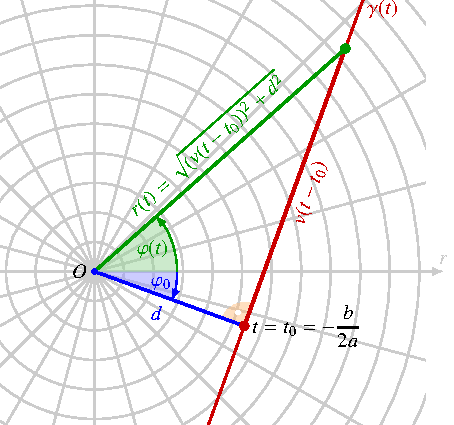
\includegraphics{chapters/100-zusammenhang/images/polargeodaete.pdf}
\caption{Geodäten in Polarkoordinaten sind Geraden.
Der Radius in Abhängigkeit vom Parameter ist $r(t)$, die Gerade
geht für den Parameterwert $t_0=-b/2a$ im kleinsten Abstand $d$
am Nullpunkt vorbei.
\label{buch:zusammenhang:geodaeten:fig:polargeodaete}}
\end{figure}
%
Schreibt man
\[
t_0=-b/2a,
\qquad
v=\sqrt{a}
\qquad\text{und}\qquad
d^2 = -\frac{b^2-4ac}{4a^2},
\]
folgt
\[
R(t)
=
(v(t-t_0))^2 + d^2
\qquad\Rightarrow\qquad
r(t)
=
\sqrt{
(v(t-t_0))^2 + d^2
}.
\]
Daraus kann man mit Hilfe des Satzes von Pythagoras ablesen, dass sich
der Punkt mit der Geschwindigkeit $v$ auf einer Geraden bewegt und
zur Zeit $t_0$ im geringsten Abstand $d$ am Nullpunkt vorbeigeht
(Abbildung~\ref{buch:zusammenhang:geodaeten:fig:polargeodaete}).
Damit lässt sich jetzt auch die Konstante $D$ bestimmen.
Aus $v=\omega d$ folgt
\[
\omega=\frac{d}{v}
\quad \Rightarrow \quad
D=\omega d^2 = \frac{d^3}{v}
\]

Aus $\dot{\varphi}=\omega = Dr^{-2} = d^3 / v r^2$
kann jetzt durch Integration auch die explizite Formel 
\[
\varphi(t)
=
\varphi_0
+
\frac{d}{v}
\int_{t_0}^t
\frac{d^2\,dt}{v^2(t-t_0)^2+d^2}
=
\varphi_0
+
\frac{d}{v}
\arctan\frac{(t-t_0)v}{d}
\]
für $\varphi(t)$ gefunden werden.

\subsubsection{Geodäten auf einer Kugeloberfläche}
In Beispiel~\ref{buch:zusammenhang:paralleltransport:bsp:kugel}
wurden die Christoffel-Symbole für Kugelkoordinaten auf einer
Kugeloberfläche berechnet.
%
% kugeldreieck.tex
%
% (c) 2025 Prof Dr Andreas Müller
%
\begin{figure}
\centering
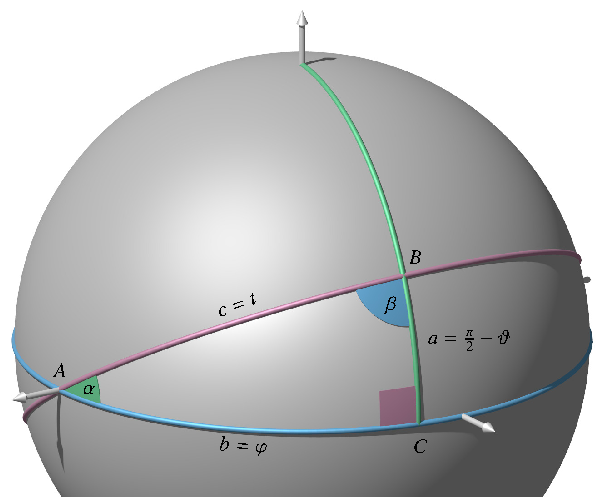
\includegraphics{chapters/100-zusammenhang/images/kugeldreieck.pdf}
\caption{Rechtwinkliges Kugeldreieck zur Parametrisierung eines
Grosskreises, der gegenüber dem Äquator um den Winkel $\alpha$ geneigt
ist.
\label{buch:zusammenhang:geodaeten:fig:kugeldreieck}}
\end{figure}
%
Damit lässt sich jetzt die Differentialgleichung für eine Geodäte auf
einer Kugel finden.
Sie ist
\begin{equation}
\left.
\begin{aligned}
\ddot{x}^1 &= \Gamma^1_{ik}\dot{x}^i\dot{x}^k
\\
\ddot{x}^2 &= \Gamma^2_{ik}\dot{x}^i\dot{x}^k
\end{aligned}
\quad
\right\}
\qquad\Rightarrow\qquad
\left\{
\quad
\begin{aligned}
\ddot{\vartheta}
&=
-\sin\vartheta\cos\vartheta \cdot \dot{\varphi}^2
\\
\ddot{\varphi}
&=
\cot\vartheta \cdot \dot{\vartheta}\dot{\varphi}.
\end{aligned}
\right.
\label{buch:zusammenhang:geodaeten:kugeldgl}
\end{equation}
Der Äquator ist durch $\vartheta=\frac{\pi}2$ definiert.
Für diesen Wert werden die Differentialgleichungen für $\varphi$ zu
\[
\ddot{\varphi}=0,
\]
die als Lösung eine lineare Funktion
$\varphi(0)=\omega t +\varphi_0$ hat.

Ein Längenkreis ist gegeben durch $\varphi=\text{const}$ oder
$\dot{\varphi}=0$, damit wird die Differentialgleichung für $\vartheta$
zu
\[
\ddot{\vartheta} = 0,
\]
die als Lösung eine lineare Funktion der Form
$\vartheta(t) = \omega t + \vartheta_0$ hat.

Andere Geodäten schneiden den Äquator, wir können ohne Beschränkung der
Allgemeinheit annehmen, dass dies für $\varphi=0$ geschieht.
In Abbildung~\ref{buch:zusammenhang:geodaeten:fig:kugeldreieck}
ist rot der Grosskreis durch den Punkt $A$ bei $\varphi=0$ dargestellt,
der den Äquator im Winkel $\alpha$ schneidet.
Als Parameter wird die Länge $c=t$ der Hypothenuse des rechtwinkligen
Dreiecks verwendet.
Der sphärische Sinussatz liefert die Beziehung
\[
\sin a : \sin \alpha
=
\sin c : \sin\gamma
=
\sin c,
\]
wegen $\sin\gamma=\sin\frac{\pi}2=1$.
Durch einsetzen der Werte aus der
Abbildung~\ref{buch:zusammenhang:geodaeten:fig:kugeldreieck}
erhalten wir
\begin{align*}
\sin\biggl(\frac{\pi}2-\vartheta\biggr) : \sin\alpha
&=
\sin t
\\
\cos\vartheta
&=
\sin\alpha \sin t
&&\Rightarrow&
\vartheta(t) &= \arccos(\sin\alpha\sin t).
\end{align*}
Für die Berechnung von $\varphi$ kann der sphärische Kosinussatz
für rechtwinklige sphärische Dreiecke in der Form
\begin{align*}
\cos c = \cos a\cos b
\quad\Rightarrow\quad
\cos\varphi\cos\biggl(\frac{\pi}2-\vartheta(t)\biggr)
&=
\cos t
\\
\cos\varphi
&= 
\frac{
\cos t
}{
\sin\vartheta(t)
}.
\end{align*}
Daraus erhalten wir als vollständige Parametrisierung des Grosskreises
\begin{equation}
\begin{aligned}
\vartheta(t)
&=
\arccos(\sin\alpha\cos t)
\\
\varphi(t)
&=
\arccos\frac{\cos t}{\sin\vartheta(t)}
\end{aligned}
\label{buch:zusammenhang:geodaeten:eqn:kugelgeodaeten}
\end{equation}

Wir prüfen jetzt durch nachrechnen, dass die Funktionen
$\vartheta(t)$ und $\varphi(t)$ gemäss
\eqref{buch:zusammenhang:geodaeten:eqn:kugelgeodaeten}
die Geodätengleichung
\eqref{buch:zusammenhang:geodaeten:kugeldgl}
erfüllen.
Dazu sind zunächst die erste und zweite Ableitung nach $t$ zu berechnen.
\begin{align*}
\dot{\vartheta}(t)
&=
-\frac{\sin\alpha\cos t}{\sqrt{1-\sin^2\alpha\sin^2 t}}
\\
\ddot{\vartheta}(t)
&=
\frac{
\sin \alpha\cos^2\alpha
}{
(1-\sin^2\alpha\sin^2t)^{\frac32}
}
\\
\dot{\varphi}(t)
&=
\end{align*}

%
% Geodäten als kürzeste Verbindungen
%
\subsection{Geodäten als kürzeste Verbindungen
\label{buch:zusammenhang:geodaeten:subsection:kuerzeste}}
Eine Kurve zwischen zwei Punkten kann in einer Karte durch eine Funktion
\(
t\mapsto x^i(t)
\)
beschrieben werden.
Die Länge dieser Kurve zwischen den Parameterwerten $t_A$ und $t_B$
ist durch das Integral
\begin{equation}
l
=
\int_{t_A}^{t_B}
\sqrt{g_{ik}(x) \dot{x}^i \dot{x}^k }
\,dt.
\label{buch:zusammenhang:geodaeten:eqn:funktional}
\end{equation}
Die Länge der Kurve ist nicht abhängig von der Parametrisierung, es ist
daher keine Einschränkung, ein festes Parameterintervall zu verwenden.

Die Lagrange-Funktion des Funktionals
\eqref{buch:zusammenhang:geodaeten:eqn:funktional}
ist 
\[
L(x^i, \dot{x}^i)
=
\sqrt{ g_{ik}(x) \dot{x}^i \dot{x}^k }.
\]
Die Wurzel führt dazu, dass die für die Euler-Lagrange-Differentialgleichung
nötigen partiellen Ableitungen von $L$ einen hässlichen Nenner haben.
Dies kann vermieden werden, indem die Unabhängigkeit der Weglänge von der
Parametrisierung ausgenutzt wird.
Verwendet man als Parameter die Weglänge, dann ist $L(x^i,\dot{x}^i)$
konstant.
Wir schreiben daher
\[
F(x^i,\dot{x}^i)
=
\frac12 L(x^i,\dot{x}^i)^2
\]
und verlangen von der Parametrisierung, dass 
\[
\frac{d}{dt} L(x^i, \dot{x}^i) = 0
\]
ist.
Die partiellen Ableitungen für die Euler-Lagrange-Differentialgleichungen
\begin{align*}
\frac{\partial F}{\partial x^l}
&=
L(x^i,\dot{x}^i)\, \frac{\partial L}{\partial x^l} (x^i,\dot{x}^i)
\\
\frac{\partial F}{\partial \dot{x}^l}
&=
L(x^i,\dot{x}^i)\, \frac{\partial L}{\partial \dot{x}^l} (x^i,\dot{x}^i).
\end{align*}
Damit wird die Euler-Lagrange-Differentialgleichung für $F$ zu
\begin{align*}
\frac{\partial F}{\partial x^l}
-
\frac{d}{dt}\frac{\partial F}{\partial \dot{x}^l}
&=
L
\frac{\partial L}{\partial x^l}
-
\frac{d}{dt}\biggl(
L
\frac{\partial L}{\partial\dot{x}^l}
\biggr)
\\
&=
L(x^i,\dot{x}^i)
\frac{\partial L}{\partial x^l}
-
\frac{dL}{dt}
\frac{\partial L}{\partial\dot{x}^l}
-
L
\frac{d}{dt}
\frac{\partial L}{\partial\dot{x}^l}.
\intertext{Da $L$ konstant ist, fällt der mittlere Term weg und es
bleibt}
\frac{\partial F}{\partial x^l}
-
\frac{d}{dt}\frac{\partial F}{\partial \dot{x}^l}
&=
L
\cdot
\biggl(
\frac{\partial L}{\partial x^l}
-
\frac{d}{dt}
\frac{\partial L}{\partial\dot{x}^l}
\biggr).
\end{align*}
Da $L$ konstant und verschieden von $0$ ist, verschwindet die rechte
Seite nur dann, wenn auch die linke Seite verschwindet.
Statt der Lagrange-Funktion $L(x^i,\dot{x}^i)$ kann also mit gleichem
Resultat die Lagrange-Funktion $f(x^i,\dot{x}^i)$ verwendet
werden.

Die partiellen Ableitungen der Lagrange-Funktion sind
\begin{align*}
\frac{\partial F}{\partial x^l}
&=
\frac12
\frac{\partial g_{ik}}{\partial x^l}
\dot{x}^i\dot{x}^k
\\
\frac{\partial F}{\partial \dot{x}^l}
&=
\frac12
g_{ik}(\dot{x}^i\delta_i^l\dot{x}^k + \dot{x}^i\dot{x}^k\delta_k^l)
=
\frac12
\bigl(
g_{lk}\dot{x}^k
+
g_{il}\dot{x}^i
\bigr).
\intertext{Für die Euler-Lagrange-Differentialgleichung ist jetzt auch
noch die Ableitung nach $t$ zu bestimmen:}
\frac{d}{dt}
\frac{\partial F}{\partial x^l}
&=
\frac12
\biggl(
\frac{\partial g_{lk}}{\partial x^s}\dot{x}^s\dot{x}^k
+
g_{lk}\ddot{x}^k
+
\frac{\partial g_{il}}{\partial x^s}\dot{x}^s\dot{x}^i
+
g_{il}\ddot{x}^i
\biggr)
\end{align*}
Damit wird die Euler-Lagrange-Differentialgleichung
\begin{align*}
0
&=
\frac{\partial F}{\partial x^l}
-
\frac{d}{dt}\frac{\partial F}{\partial\dot{x}^l}
\\
&=
\frac12
\biggl(
\frac{\partial g_{ik}}{\partial x^l}
\dot{x}^i\dot{x}^k
-
\frac{\partial g_{lk}}{\partial x^s}\dot{x}^s\dot{x}^k
-
\frac{\partial g_{il}}{\partial x^s}\dot{x}^s\dot{x}^i
\biggr)
-
\frac12
g_{lk}\ddot{x}^k
-
\frac12
g_{lk}\ddot{x}^k
\\
&=
\frac12
\biggl(
\frac{\partial g_{ik}}{\partial x^l}
\dot{x}^i\dot{x}^k
-
\frac{\partial g_{lk}}{\partial x^i}\dot{x}^i\dot{x}^k
-
\frac{\partial g_{il}}{\partial x^k}\dot{x}^k\dot{x}^i
\biggr)
-
g_{lk}\ddot{x}^k
\\
&=
\frac12
\biggl(
\frac{\partial g_{ik}}{\partial x^l}
-
\frac{\partial g_{lk}}{\partial x^i}
-
\frac{\partial g_{il}}{\partial x^k}
\biggr)
\dot{x}^i\dot{x}^k
-
g_{lk}\ddot{x}^k
\\
&=
-\Gamma_{l,ik} \dot{x}^i\dot{x}^k
-
g_{lk} \ddot{x}^k
\end{align*}
Multipliziert man dies mit den Einträgen $g^{jl}$ der inversen
Matrix von $g$ und summiert über $l$, ergibt sich
\[
0
=
g^{jl}\Gamma_{l,ik}\dot{x}^i\dot{x}^k+g^{jl}g_{lk}\ddot{x}^k
=
\Gamma^j_{ik}\dot{x}^i\dot{x}^k + \delta^j_k\ddot{x}^k
=
\Gamma^j_{ik}\dot{x}^i\dot{x}^k + \ddot{x}^j.
\]
Die Euler-Lagrange-Differentialgleichung für das Weglängenfunktional
ist also die Differentialgleichung für Geodäten.

%
% Zusammenhang
%
\section{Zusammenhang
\label{buch:zusammenhang:section:zusammenhang}}

%
% Kovariante Ableitung
%
\subsection{Kovariante Ableitung
\label{buch:zusammenhang:zusammenhang:subsection:kovarianteableitung}}

%
% Strömungsgleichungen
%
\section{Strömungsgleichungen
\label{buch:zusammenhang:section:stroemungsgleichungen}}




